\section{\emph{Build Server}}
\label{sec:buildserver}
Dieser Abschnitt behandelt die Infrastruktur des \emph{Build}-Server in Openshift. Der \emph{Build}-Server wird innerhalb eines Openshift Projekts organisiert. Nachdem der \emph{Build}-Server erstellt wurde, muss das Nexus Password abgeändert werden und die Release \emph{Policy} beim Maven \emph{Repository /maven-releases} auf \emph{Allow Redeploy} umgestellt werden.
\subsection{\emph{Templates}}
\label{sec:openshift-templates}
Dieser Abschnitt behandelt die Openshift \emph{Templates}, welche die Integration der einzelnen Services innerhalb der \emph{Build}-Server Infrastruktur in Openshift spezifizieren. Die Openshift \emph{Templates} beinhalten alle Definitionen wie z.B. \emph{Build}-Konfigurationen und \emph{Deployment}-Konfigurationen, die Aspekte der \emph{Core Conepts}\footnote{\url{https://docs.openshift.com/container-platform/3.5/architecture/core_concepts/index.html}} von Kubernetes und Openshift sind. \\

Die folgende Auflistung beschreibt die implementierten \emph{Templates}:
\begin{enumerate}
	\item Im \emph{Template} \textbf{\emph{jenkins-slaves.yml}} werden die für Jenkins zur Verfügung gestellten \emph{Slave-Container} spezifiziert.
	\item Im \emph{Template} \textbf{\emph{jenkins.yml}} wird der Jenkins Service spezifiziert.
	\item Im \emph{Template} \textbf{\emph{nexus.yml}} wird der Nexus3 Service spezifiziert.
	\item Im \emph{Template} \textbf{\emph{pipeline.yml}} wird eine Openshift \emph{Build}-Konfiguration Pipeline spezifiziert.
\end{enumerate}

\ \subsection{Skripte}
Dieser Abschnitt behandelt die Skripten, die für das Verwalten des \emph{Clusters} verwendet werden. Mit der Applikation \emph{oc} kann mit einem lokalen oder entfernten \emph{Cluster} interagiert werden. Damit der \emph{Build Server} einfach erstellt und gelöscht werden kann, sind für die einzelnen Services und für den \emph{Build Server} selbst
Skripte erstellt worden, die alle nötigen Funktionalitäten beinhalten.\\

Auf dem Level der Skripten wird eine Datei namens \emph{.openshift-env} und \emph{.openshift-secret-env} erwartet. Die Datei \emph{.openshift-env} definiert Umgebungsvariablen wie z.B. Service und \emph{Secret} Namen, die über mehrere Skripten verwendet werden. Die Datei \emph{.openshift-secret-env} definiert Umgebungsvariablen, welche die Passwörter für die \emph{Secrets} definieren. Die folgende Auflistung beschreibt die implementierten \emph{Skripte}:
\begin{enumerate}
	\item Im \emph{Skript} \textbf{\emph{openshift-jenkins.sh}} sind alle Jenkins Service und Jenkins \emph{Slave} spezifischen Funktionen implementiert.
	\item Im \emph{Skript} \textbf{\emph{openshift-nexus.sh}} sind alle Jenkins Service und Jenkins \emph{Slave} spezifischen Funktionen implementiert.
	\item Im \emph{Skript} \textbf{\emph{openshift-buildserver.sh}} sind alle Funktionalitäten für das Verwalten des \emph{Build Servers} implementiert.
	\item Im \emph{Skript} \textbf{\emph{openshift-secrets.sh}} sind alle Funktionalitäten für das Verwalten von \emph{Secrets} implementiert. Siehe Abschnitt \ref{sec:buildserver-secrets} für eine genauere Beschreibung der verwendeten \emph{Secrets}.
\end{enumerate}
\ 
\subsection{\emph{Update} Szenarien}
\label{sec:buildserver-updates}
Dieser Abschnitt behandelt die \emph{Update}-Szenarien für den \emph{Build Server}. Es gibt folgende drei Szenarien für das Updaten des \emph{Build Servers}:

\begin{enumerate}
	\item Bei \textbf{\emph{Änderung der Quelltexte}} wie \emph{S2I Builds}\footnote{\url{https://github.com/openshift/source-to-image}} oder \emph{Dockerfiles}, muss der Docker \emph{Container} neu gebaut und der Service neu eingespielt werden.
	\item Bei \textbf{\emph{Änderung der Konfigurationen}}, muss der Service gegebenenfalls neu gebaut und eingespielt werden.
	\item Bei \textbf{\emph{Änderung der Docker Images}}, die Services beinhalten oder Basisimages darstellen, muss der Service neu gebaut und eingespielt werden.
\end{enumerate}
Diese drei \emph{Update}-Szenarien können einfach in Openshift abgebildet werden, da Openshift alle nötigen \emph{Trigger}-Mechanismen zur Verfügung stellt, damit diese Änderung eingespielt werden können. 
\newpage

Openshift erlaubt es bei \emph{Deployment}-Konfigurationen und \emph{Build}-Konfigurationen \emph{Trigger}\footnote{\url{https://docs.openshift.com/container-platform/3.5/dev_guide/builds/triggering_builds.html}} zu definieren. Folgende \emph{Trigger}-Typen werden bereitgestellt:
\begin{enumerate}
	\item\textbf{\emph{Github}} ist ein \emph{Trigger}-Typ, der auf Github \emph{Webhooks} regiert.
	\item\textbf{\emph{ImageChange}} ist ein \emph{Trigger}-Typ, der auf Änderungen des angegebenen Docker Images regiert.
	\item\textbf{\emph{ConfigChange}} ist ein \emph{Trigger}-Typ, der auf Änderungen der Konfiguration eines Openshift Artefaktes regiert.
\end{enumerate}

\begin{figure}[H]
	\centering
	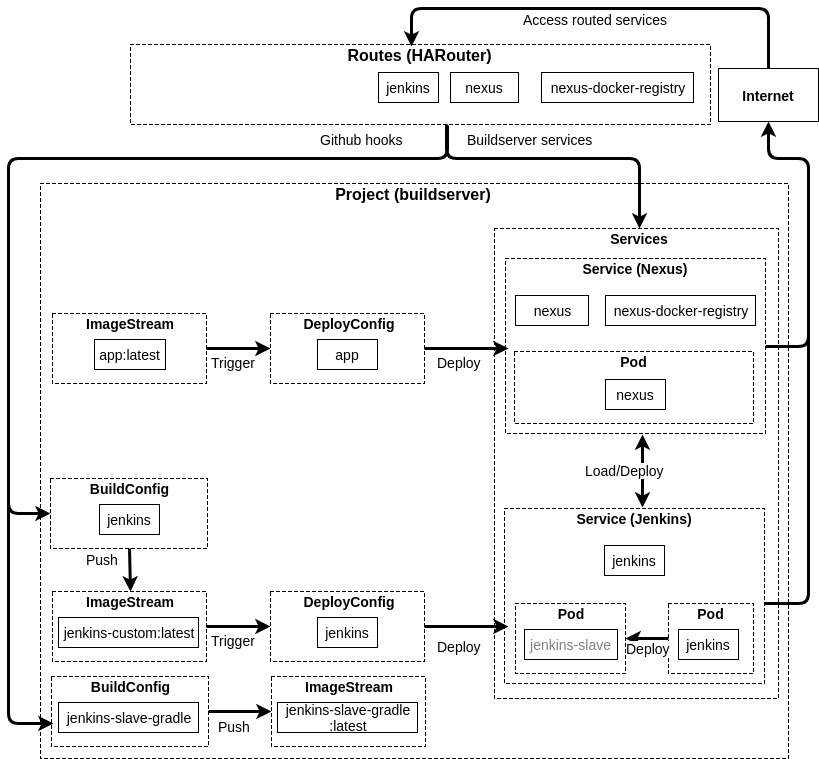
\includegraphics[scale=0.55]{logos/architecture-diagram-buildserver.jpg}
	\caption{\emph{Build Server} Architektur}
	\label{fig:architecture}
\end{figure}
\ \newpage
Die Abbildung \ref{sec:buildserver} zeigt die Architektur der \emph{Build}-Server Infrastruktur, sowie den Ablauf der Prozesse, die von den Triggern ausgelöst werden. Die folgenden Abschnitte beschreiben die verwendeten \emph{Trigger}-Typen näher.
\subsubsection{Github \emph{Trigger}}
Dieser Abschnitt behandelt den verwendeten \emph{Github Trigger}, der dazu verwendet wird, um die Docker Images bei Quelltextänderungen neu zu bauen und den Service zu aktualisieren.\\

Beim Jenkins Docker Image und den \emph{Slave} Images, wird bei einem \emph{Push}, das Image neu gebaut.

\begin{minted}{yaml}
triggers:
- type: "GitHub"
  github:
  secret: "<SECRET_NAME>" # Obfuscates the webhook url, not really a secret
\end{minted}
Wenn ein Github \emph{Trigger}-Typ definiert wurde, wird von Openshift eine \emph{Webhook Url} erstellt, die bei Github registriert werden muss.

\subsubsection{\emph{ImageChange Trigger}}
Dieser Abschnitt behandelt den verwendeten \emph{ImageChange Trigger}, der dazu verwendet wird, um bei Änderungen der Docker Images, die über \emph{ImageStream} repräsentiert werden, die Docker Images der Service neu zu bauen.\\

Alle verwendeten Services definieren einen \emph{ImageChange Trigger}. Änderungen an den Docker Images, die über \emph{ImageStreamTags} referenziert werden, werden nur bei Docker \emph{Registries} in Version 2 unterstützt, da Docker \emph{Registries} in Version 1 es nicht erlauben Images eindeutig zu identifizieren.
\begin{minted}{yaml}
triggers:
- type: "ImageChange"
  imageChange:
  automatic: true
  containerNames:
    - "<CONTAINER_NAME_USING_IMAGE>" 
  from:
    kind: "ImageStreamTag"
    name: "<IMAGE_STREAM_NAME:IMAGE_STREAM_TAG_NAME>"
\end{minted}

\subsubsection{\emph{ConfigChange Trigger}}
Dieser Abschnitt behandelt die verwendeten \emph{ConfigChange Trigger}, die auf Änderungen der Konfiguration des Openshift Artefakts reagieren.\\

Alle definierten Konfigurationen verwenden den \emph{ConfigChange Trigger}, der bei Änderungen einer Konfiguration z.B. einen neuen \emph{Build} oder ein neues \emph{Deployment} auslöst.
\begin{minted}{yaml}
triggers:
  - type: "ConfigChange"
\end{minted}
